\subsection{erstes}
\[
  P_a=t^2\partial_t^2+t\partial_t+(t^2-n^2)=\sum_{k=0}^2\sum_{l=0}^2
  \alpha_{kl}t^l\partial_t^k
\]

Mit: $\alpha_{2,2}=1$, $\alpha_{1,1}=1$, $\alpha_{0,2}=t^2$ und
$\alpha_{0,0}=n^2$

$
P_a=t^2\partial_t^2+t\partial_t+(t^2-n^2) \Rightarrow 
\begin{cases}
  k=2,l=2 & \Rightarrow u\leq k=2, v\geq l-k=0\\
  k=1,l=1 & \Rightarrow u\leq 1, v\geq 0\\
  k=0,l=0 & \Rightarrow u\leq 0, v\geq 0\\
  k=0,l=-2 & \Rightarrow u\leq 0, v\geq 2\\
\end{cases}
$

\begin{center}
  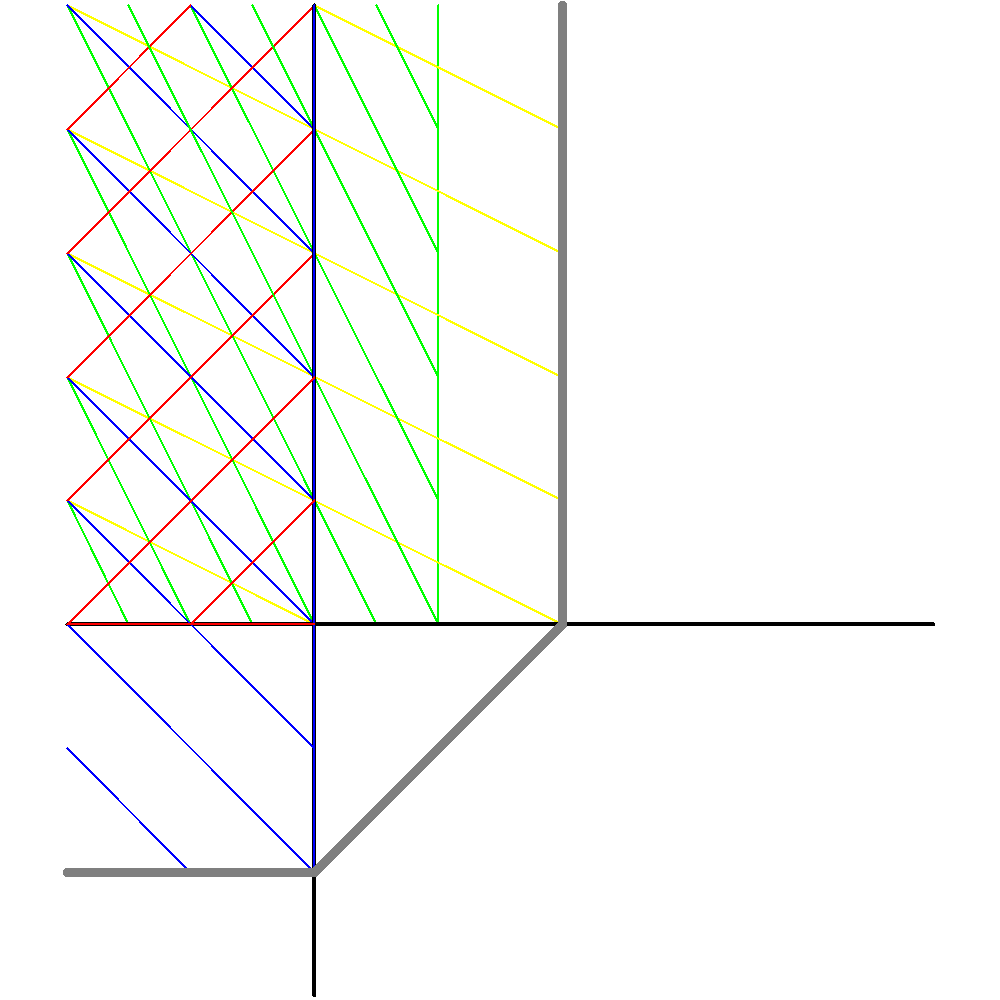
\includegraphics[width=6cm]{img/a.png}
\end{center}
also $\slopes(P_a)=\{1\}$

% vim: set ft=tex :
